% !TEX program = lualatex
\documentclass[../../main.tex]{subfiles}
\begin{document}

There are some fundamental things that is largely the same between the solvers which will be explained here. In each dedicated section for the solver any changes to this will be explained further. A few key details about the state space is also given. \\

The state space of Sokoban has a branching factor of 4 as the robot can move to non-diagonal adjacent tiles. The state space itself is finite.

Storing a state which includes all the box positions stored in a list and the player position is required to have 				sufficient 	information about a state. State and node is used interchangeably but refers to the same concept. The state is stored in a dictionary where the key is a list of strings of the levels layout. The node object itself is stored as the value. It is highly desirable that a state has a unique board position and a node also stores what node its parent and children are. \\

When a path is constructed it has to be accounted for that there is a branching factor of 4 meaning that the delta move is either -1 or 1 in the x-axis or -1, 1 in the y-axis. Depending on what the delta move value is a character representing the direction will be appended to the solution string. If a box is moved in a specific move that character will be uppercase. \\

The problem is created in the same manner in both solvers. It is required that a solution is defined which is that all the boxes in the level are on a goal. The solution is then compared to the hash as every node is visited. Goals, boxes and the player is also created based on the level string. Hashes, which is the dictionary key are also created in the same way between the solvers. 

Generating children follows the same idea, however, there is some important differences for the A-star implementation which will be discussed in its own section. When generating children of a node, a new child node is found by adding each of the four possible moves to the node's current position. It is also here some basic deadlock functionality has been implemented to reduce the amount of nodes that there is no use for. The simple deadlock detection is shown in the figure below.

\begin{figure}[h]
	\centering

	\subfloat[][Deadlock showcase]{
		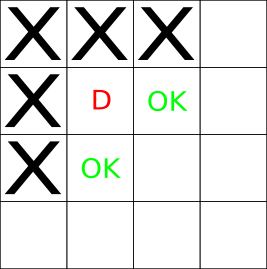
\includegraphics[width=0.4\linewidth]{images/basic_deadlock_detection.png}
	\label{fig:images/basic_deadlock_detection}
	}
	\caption{States like D are those that will be pruned}
	\label{fig:basic_deadlock_detection}
\end{figure}

What the figure above shows is only valid if the position of D is not a goal. To be clear it is the two X's that touch D non-diagonally that tells whether the can is in a deadlock position. In the section about breadth first search there will be a comparison of no deadlock detection and deadlock detection enabled.

\end{document}
